\section{Analog to digital conversion}
A Honeywell SS495 Hall effect sensor has been used into the project to detect the position of the permanent magnet. When fed with 5Vdc, the sensor has a linear output wrt the sensed magnetic field, being 2.5V with no field, 0V with strong negative magnetic field and 5V with strong positive magnetic field. The coil has been turned so that it emits negative magnetic field, to which the permanent magnet will respond, if positioned so that it is attracted, with another negative magnetic field.

The Stellaris microcontroller has a 12-bit ADC device, which can be configured to sample from a sequence of channels with manual or event-based trigger. In this project, the ADC has been used to periodically sample the Hall effect sensor on pin E3 of the microcontroller. A timer is set up into the microcontroller with a 10kHz frequency as a trigger for the ADC conversion. Two considerations have been done: first, the sensor's output can be amplified in order to increase the reading's precision. In particular, and with a little margin, a gain of 1.3 on the sensor's output can bring the interesting output range (0-2.5V) to the full ADC range (0-3.3V). This has been implemented with a non-inverting amplifier stage using a LM318N operational amplifier. The other and most important thing to consider is that, if magnetic field with the opposite direction is applied, the sensor output is in the range 2.5-5V. This would for sure damage the ADC input pin, as the ADC is fed with a 3.3V reference and can't stand higher input voltages. Thus, a protection stage is applied, with a 100$\Omega$ resistor going to ground through a 3.3V zener diode. If the zener diode is off the resistor does not influence the reading, while if the output grows to more than 3.3V the diode will turn on and limit the output voltage to 3.3V, thus protecting the ADC pin.

\begin{figure}[htbp]
\centering
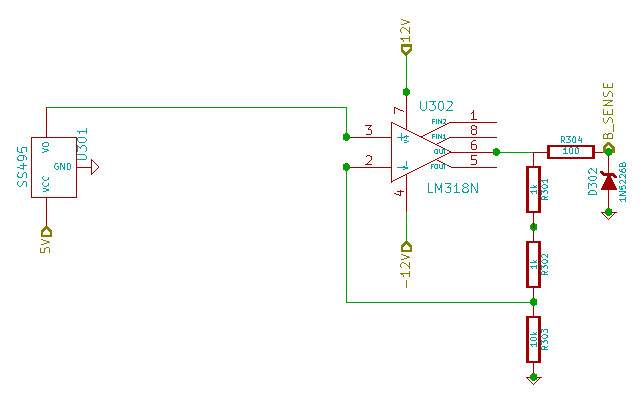
\includegraphics[width=4in]{Graphics/inputStage}
\caption{Schematics for the SS495 analog-to-digital input stage}
\end{figure}
